\section{Overview}

In order to insert additional code
and data into an executable, additional space needs to be allocated within the executable in a way that they
will, at load-time, be treated as code and data respectively. Most compilers produce an ELF executable whose
structure is similar to that shown in Figure \ref{Figure:Executable}. By
convention, most executables use only two loadable segments and some of the Linux
implementations, such as FreeBSD, only allow two loadable segments. Thus, it is
preferable to incorporate instrumentation text and data into the
existing text and data segments of the application. The default in most
compilers is to place the text segment prior and adjacent to the data segment.

\subsection{Code and Data Discovery}
In a typical ELF executable, code and data can reside together in the text section of the executable due to several reasons, including
the storage of branch target locations (e.g. for a jump table as a result of switch statements) or small data structures 
that provide convenient and efficient look-up of data such as identifiers and descriptors. 
For the correctness of the executable after instrumentation, it is extremely important to identify  the parts of the text 
section that are code and the parts that are data. Mishandling of already existing data in text section as code 
may result in a different behavior than the original behavior of the uninstrumented run, especially, 
if the instrumentation tool chooses to modify or relocate the part that data resides 
to serve the needs of the instrumentation task and when the data at that location is referenced. 
Such change in program behavior may cause application failure due to some unexpected change in control flow 
or some state condition that is checked by the program.
However, the corruption in data in text section might silently manifest itself by modifying the output of the
program, which would be the undesirable behavior.  Alternatively, if we mistakenly treat some code as data in text section, we may skip
to insert instrumentation code into this area or we might perform analysis that should be reserved for
data alone. While this is almost certainly preferable to the situation where we treat data as code, it
is ideal to avoid both situations completely for instrumentation task to be complete and correct.

To determine which parts of the text sections are functions that are eligible to be subject for our code discovery algorithm, 
we use the program's symbol table entries \textbf{(COMMENT: The minimal or -g is required)}. Our code discovery algorithm
consists of two phases; control-driven disassembly backed up by linear disassembly. During the control driven disassembly, 
we follow all understandable control paths starting at a function's entry point. If a problem is encountered such as 
\textbf{(COMMENT some problematic examples)}, 
we fall back to naive disassembly. During the naive disassembly, we disassemble each instruction in the order it appears in the
function starting at a function's entry point. If a problem is encountered such as \textbf{(COMMENT some problematic examples)}, 
we tag the function uninstrumentable. For our code discovery algorithm, we start with the 
\textbf{(COMMENT: Which function or entry point we start with???)} function in the executable. 

Even though our code discovery algorithm identifies most of the control flow and instructions, it may fail to 
identify the complete control flow and instructions for some functions.  Problems that can be encountered during code discovery
are situations where an unknown opcode is encountered, where control jumps to the
middle of an instruction we've already disassembled, or if control leaves the boundaries of the function. In most
cases control-driven disassembly is sufficient to disassemble the entirety of a function, and in most cases control-driven
disassembly is a straightforward process because control either falls through to the following instruction 
or the location of a branch target is embedded entirely within the instruction itself. But there are also cases
where an indirect branch is used, the target resides either at a fixed address (possibly with some offset),
the address that resides in a register, or the address that is at a location given by a register. The latter two cases are difficult to resolve
without runtime information since the computation of the target address can be arbitrarily complex and can span function
boundaries. Nevertheless, we perform a peephole examination of the preceeding instructions and can determine 
the address in most of the cases.

Fortunately, simple calculations are all that most compilers use to determine targets for jump tables, one of the more common
uses of an indirect branch. Often an offset is added to a fixed location to determine where the data comprising the branch target
resides. Therefore, we treat such a fixed address as the first entry in a table whose entries are treated either as addresses or as offsets.
We then make an iterative pass over this table to determine the target for each entry in the jump table, stopping when we find a value in the
table that yields an address that is outside the scope of the function.

\textbf{(COMMENT : Put an example of GNU compiler Jump table entry).}

\subsection{Additional Code and Data Insertion}

%In the design of PIX we use static binary instrumentation because it is more efficient
%due to the fact that it generates a persistent instrumented executable 
%that can be run at a later time. When the instrumented executable is
%run, the extra instrumentation code is run
%in addition to the original code of the program. 

In PIX, we prepend the instrumentation text to the existing text
segment\footnote{The amount of space allocated prior to the text section is
controlled by the linker variable \_\_executable\_start. We have seen cases
where the system does not provide enough space prior to the text segment by
default, in which case we provide a set of tools that produces a modified linker
script that provides up to 128MB of space.} and append the instrumentation data to the
data segment (as shown in Figure \ref{Figure:Executable}). This
scheme has the added benefit of causing no immediate disturbance to the
addresses of the original data and most of the original text segments of the program.

\begin{figure}[ht]
\centering
\caption[Optional caption for list of figures]{\subref{Figure:OrigExecutable} and \subref{Figure:InstExecutable} show the prepending
of instrumentation text to the existing text, and the prepending of instrumentation data to the existing data respectively.}
\subfigure[Layout of an unmodified ELF file.]{
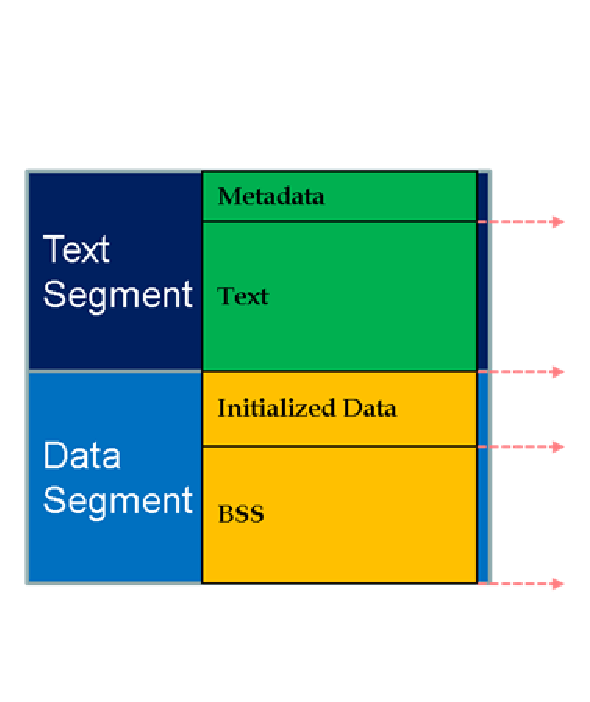
\includegraphics[scale=0.65]{executablep1.eps}
\label{Figure:OrigExecutable}
}
\subfigure[Layout of an instrumented ELF file.]{
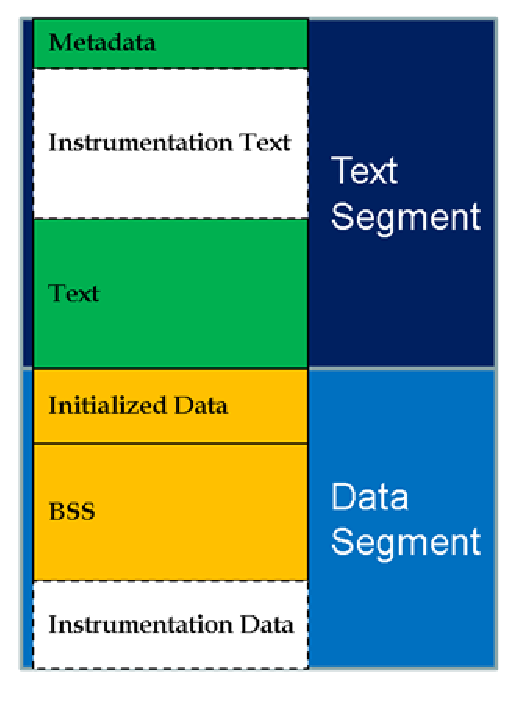
\includegraphics[scale=0.65]{executablep2.eps}
\label{Figure:InstExecutable}
}
\label{Figure:Executable}
\end{figure}

The instrumentation text in PIX contains several types of additional code. The first
is the code that accomplishes the instrumentation tasks as well as any bookkeeping code.
When control is transferred from the application to the
instrumentation code, it is necessary to maintain the machine state of
the application to preserve its original behavior. This machine state
can contain anything modified by the instrumentation code, but in practice is
usually limited to a relatively limited set of registers but in some cases includes
some information about the call stack. The code sequence, called a \textit{trampoline} \cite{buck2000api}, 
saves any machine state that will be destoryed, performs the instrumentation task, restores
the machine state after the instrumentation, executes the
original instructions that were displaced by the initial control transfer,
and finally restoring control to the original code. Since we are using a jump instruction at the instrumentation point, the
instrumentation code has no information about where control was transferred from
(as might be the case if we used the more heavyweight call instruction). Hence
each instrumentation point uses its own trampoline so that the location of the
instrumentation point can be hard-coded into an unconditional branch instruction
at the end of the trampoline.

Since some instrumentation tools may need additional data to support the inserted instrumentation code,
PIX provides mechanisms to add and initialize additional data in to the executable.
The instrumentation text also includes code to initialize this additional data for use by the
instrumentation tool. Recall from Figure \ref{Figure:Executable} that the instrumentation
data was appended to the end of the application's data segment, after the
application's uninitialized data section (BSS section) in order to preserve the application's 
original addresses. The initialized data and BSS
sections of the data segment are usually implemented by declaring the size of
the data segment in the executable to be smaller than the size of the data
segment in memory. According to the ELF specification\cite{standard1995executable}, the extra part of any
segment whose memory size is greater than its file size should be filled with
zeroes by the loader. Hence most programs just increase the size of the data
segment in memory by the size of the BSS section in order to get a large
area that is filled with zeroes, which  is reserved for uninitialized data. Since we
would like to use the area following the BSS section for additional
data for the instrumentation tool, we can either explicitly include the entire
segment's contents in the executable file or we can implicitly reserve this area.
Since the BSS section can be very large and explicit inclusion of its contents
would bloat the  executable file, we use the implicit
technique to reserve this section for instrumentation data. We therefore
temporarily store the instrumentation data with the instrumentation text in the
executable as well as some code to copy it to the appropriate location in the
data segment once the program starts.
